% !TEX encoding = UTF-8 Unicode
\documentclass[hidelinks,9pt, oneside]{extarticle}     % use for two column: ,twocolumn
\usepackage{hyperref}
\usepackage{fancyvrb}
  \fvset{tabsize=4}%changes tab spacing in verbatim from 8 to 4
%\usepackage{geometry}                    % See geometry.pdf to learn the layout options. There are lots.
%\geometry{letterpaper}                       % ... or a4paper or a5paper or ...
%\usepackage[pass,letterpaper]{geometry}
\usepackage[margin=2cm,letterpaper]{geometry}
%\geometry{landscape}                    % Activate for for rotated page geometry
\usepackage[parfill]{parskip}        % Activate to begin paragraphs with an empty line rather than an indent
\usepackage{graphicx}        % Use pdf, png, jpg, or eps? with pdflatex; use eps in DVI mode
                  % TeX will automatically convert eps --> pdf in pdflatex
\usepackage{amssymb}
\usepackage{tikz,adjust box}      %adjustbox is for figures that span 2 columns
\usepackage{dashrule}        %used to make dashed line in text
\usepackage{amsmath}
\usepackage{fancyhdr}        %used to put draft in header
%\pagestyle{fancy}          %
\DeclareMathOperator{\arcsec}{arcsec}  %arcsec, arccsc... not defined inamsmath
\usepackage{exsheets}        %Formats questions and solutions
\SetupExSheets{solution/print=false,question/name={},solution/name={}}    %Solutions on or off;
\SetupExSheets{headings=runin}    % Puts questions next to number
\SetupExSheets{use-classes={easy,medium,hard}}  % Print questions by difficulty level
\usepackage{natbib,endnotes}      %Bibliography and Footnote to endnote
\usepackage{title sec}        %Format section titles to include horizontal line
%\usepackage{enumitem}        %Allow lists to be a, b, c and not 1, 2, 3
\usepackage{enumerate}
\usepackage{epigraph}




%\renewcommand{\theenumi}{\alph{enumi}}
%\setenumerate[0]{label=(\alph*)}
\let\footnote\endnote
\titleformat{\section}
  {\normalfont\Large\bfseries}{\thesection}{1em}{}[{\titlerule[0.8pt]}]
\newcommand{\calc}{\protect\includegraphics[height = 2.5ex]{images/calc.png}}
%%%%%%%%%%%%%%%%%%%%%%%%%%%%%%%%%%%%%%%%%%%%
%%%%%%%%Convert paragraph to subsubsubsection %%%%%%%%%%%%%%%%
\makeatletter
\renewcommand\paragraph{\@startsection{paragraph}{4}{\z@}%
            {-2.5ex\@plus -1ex \@minus -.25ex}%
            {1.25ex \@plus .25ex}%
            {\normalfont\normalsize\bfseries}}
\makeatother
\setcounter{secnumdepth}{4} % how many sectioning levels to assign numbers to
\setcounter{tocdepth}{4}    % how many sectioning levels to show in ToC
%%%%%%%%%%%%%%%%%%%%%%%%%%%%%%%%%%%%%%%%%%%%%%

%%%%%%Macros: begin question cntrl command Q or S for solution
%\title{An Introduction to the Tex Document Preparation System}
%\subtitle{Graphs, Diagrams, Presentations and Documents}
%\author{Frank Briody}
%\institute[PHS] % (optional)
% {
%   Prospect High School\\
%   Mt. Prospect, IL
% }

% \date[MMC 2019] % (optional)
% {MMC Conference, January 2019}
%\chead{}
\begin{document}

\begin{titlepage} % Suppresses headers and footers on the title page
  \centering % Centre everything on the title page
  \scshape % Use small caps for all text on the title page
  \vspace*{\baselineskip} % White space at the top of the page
  %------------------------------------------------
  %  Title
  %------------------------------------------------
  \rule{\textwidth}{1.6pt}\vspace*{-\baselineskip}\vspace*{2pt} % Thick horizontal rule
  \rule{\textwidth}{0.4pt} % Thin horizontal rule
  \vspace{0.74\baselineskip} % Whitespace above the title

  {\LARGE THE LINEAR REGRESSION PROCESS} % Title

  \vspace{0.75\baselineskip} % Whitespace below the title
  \rule{\textwidth}{0.4pt}\vspace*{-\baselineskip}\vspace{3.2pt} % Thin horizontal rule
  \rule{\textwidth}{1.6pt} % Thick horizontal rule

  \vspace{2\baselineskip} % Whitespace after the title block
  %------------------------------------------------
  %  Subtitle
  %------------------------------------------------
  From Generation to Interpretation % Subtitle or further description

  \vspace*{3\baselineskip} % Whitespace under the subtitle
  %------------------------------------------------
  %  Editor(s)
  %------------------------------------------------
  Presented By

  \vspace{0.5\baselineskip} % Whitespace before the editors
  {\scshape\Large Frank Briody \\ } % Editor list
  \textit{frankbriody@gmail.com}\\ %
  \vspace{0.5\baselineskip} % Whitespace below the editor list
  \textit{Prospect High School \\ Mt. Prospect, IL \\ } % Editor affiliation

  
\includegraphics[width=.1\textwidth]{img/phs_logo.png}

  \vfill % Whitespace between editor names and publisher logo
  %------------------------------------------------
  %  Publisher
  %------------------------------------------------
  %\plogo % Publisher logo
  \vspace{0.3\baselineskip} % Whitespace under the publisher logo
  2022 % Publication year
  {\large MMC Conference of Workshops}\\[.1in] % Publisher
  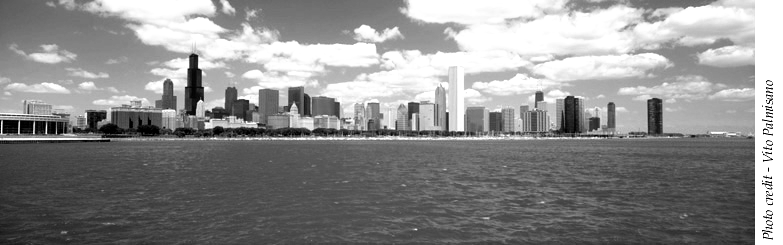
\includegraphics[width=\textwidth]{img/mmc_logo.png}
\end{titlepage}

\tableofcontents
  %\maketitle
\begin{centering}
  \date{\today}
\end{centering}


\newpage


%\epigraph{Put quote here. There is only one large computer program I have used in which there are to a decent approximation 0 bugs: Don Knuth's TeX}{\textit{ -- Jaap Weel}}

\colorbox{black}{{\bf \textcolor{white}{\textsf{The Story}}}}\\
\fbox{%
\parbox{\linewidth}{%
A statistics teacher gives a quiz to a class. The scores were 2, 4, 6, 8, and 15 with one student being absent. Absent student returns the next day...\\
\textbf{Student}: How am I going to do on the quiz?\\
\textbf{Teacher}: Well, the class average was...
}%
}

%%%%%%%%%%%
%Prequel%%%%
%4_2_Notes_21%
%%%%%%%%%%%
\section{Prologue: Standard Deviation}

How much variability, on average, is there around the mean?

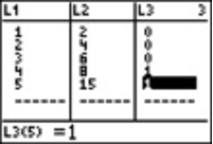
\includegraphics[width=.2\textwidth]{img/4_2_1}
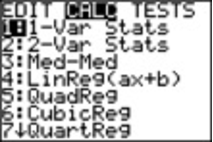
\includegraphics[width=.2\textwidth]{img/4_2_2}
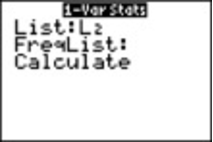
\includegraphics[width=.2\textwidth]{img/4_2_3}
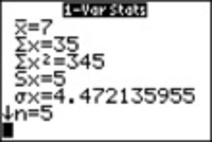
\includegraphics[width=.2\textwidth]{img/4_2_4}
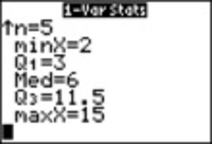
\includegraphics[width=.2\textwidth]{img/4_2_5}


\begin{table}[ht]
\large
%\centering
\huge{%
\begin{tabular*}{6cm}[h]{cccc}
Score & Deviation & Squared Deviation & \hspace{1.5in} \\
$x$ &  &  & \quad \\
\cline{1-4}
2 & \quad & \quad & \quad\\
4 & \quad & \quad & \\
6 & \quad & \quad & \\
8 & \quad & \quad & \\
15 & \quad & \quad &
\end{tabular*}
}
\end{table}

\newpage

%%%%%%%%%%%
%MAIN 1%%%%
%5_2_Notes%
%%%%%%%%%%%


\colorbox{black}{{\bf \textcolor{white}{\textsf{The Story Part 2}}}}\\
\fbox{%
\parbox{\linewidth}{%
A statistics teacher gives a quiz to a class. The scores were 2, 4, 6, 8, and 15 with one student being absent. After surveying the class, the teacher knows the hours studied were 1, 2, 3, 4 and 5, respectively. Absent student returns the next day...\\
\textbf{Student}: How am I going to do on the quiz?\\
\textbf{Teacher}: That depends - how long did you study?
}%
}

\section{Getting Least Squares Line of Best Fit} % (fold)
 % \label{}
 % \subsection{From Calculator}
 %   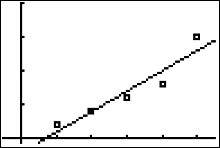
\includegraphics[width=.15\textwidth]{img/5_scat}

 \begin{table}[ht]
 \centering
 \begin{tabular*}{6cm}[h]{llllll}
 Hours ($x$) & 1 & 2 & 3 & 4 & 5   \\
 Score ($y$) & 2 & 4 & 6 & 8 & 15
 \end{tabular*}
 \end{table}

\subsection{From Summary Statistics} % (fold)
\label{sub:from_summary_statistics}
{\bf Formulas} (given): $\hat{y} = a + bx$\quad\quad$b = r\frac{s_y}{s_x}$\quad\quad$a=\bar{y}-b\bar{x}$\\[.2in]
{\bf Descriptive Statistics}: x, y\\
\verb|Variable  N  N*   Mean  SE Mean  StDev  Minimum     Q1  Median     Q3  Maximum|\\
\verb|x         5   0  3.000    0.707  1.581    1.000  1.500   3.000  4.500    5.000|\\
\verb|y         5   0   7.00     2.24   5.00     2.00   3.00    6.00  11.50    15.00|\\[.1in]
{\bf Correlations}: x, y \\
\verb|Pearson correlation of x and y = 0.949|\\
\verb|P-Value = 0.014|\\[.5in]

% subsection from_summary_statistics (end)


\newpage

\subsection{From Output} % (fold)
\label{sub:from_output}
%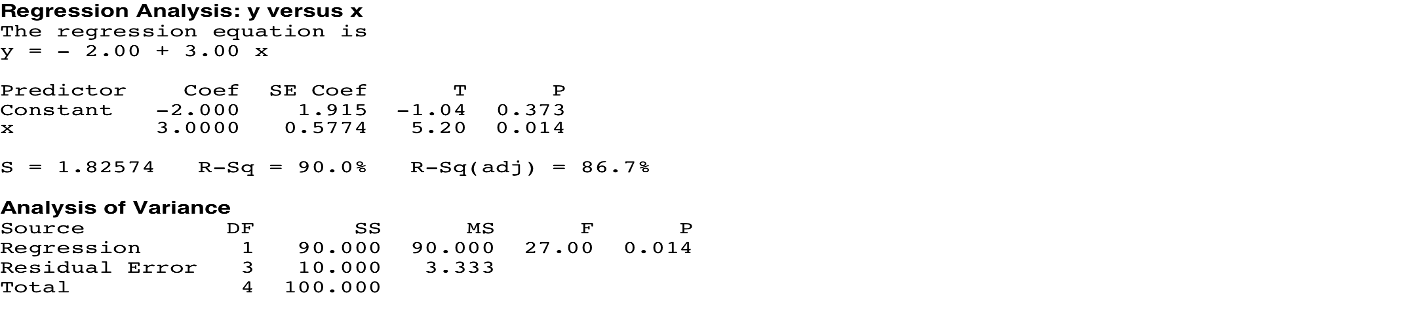
\includegraphics[width=1\textwidth]{img/5_RegOut}\\[.25in]

{\bf Regression Analysis: y versus x}\\
\verb|The regression equation is|\\
\verb|y = - 2.00 + 3.00 x|\\
\verb||\\
\verb|Predictor     Coef   SE Coef         T       P|\\
\verb|Constant    -2.000     1.915     -1.04    0.373|\\
\verb|x           3.0000    0.5774      5.20    0.014|\\
\verb||\\
\verb|s = 1.82574    R-sq = 90.0%    R-Sq(adj) = 86.7%|
\verb||\\

{\bf Analysis of Variance}\\
\verb|Source           DF         SS        MS        F        P|\\
\verb|Regression        1     90.000    90.000    27.00    0.014|\\
\verb|Residual Error    3     10.000     3.333|\\
\verb|Total             4    100.000|\\

\vspace{3in}
\section{Interpretation} % (fold)
\label{sub:interpretation}
\subsection{Slope}
Slope represents the  \textbf{predicted} change in response associated with each unit increase in the explanatory variable, \textbf{on average}.\\[.25in]
\subsection{Y-Intercept}
Y-intercept is the predicted value when the explanatory $(x)$ is 0. [Often the y-intercept is useless due to \textit{extrapolation}.]
% subsection interpretation (end)


\newpage

%%%%%%%%%%%
%MAIN 2?%%%%
%5_3_Notes%
%%%%%%%%%%%

\section{Predicted Values and Residuals}
  %\centering
  $\hat{y}=-2+3x$
  \begin{table}[ht]
  \Huge
  %\centering
  \begin{tabular*}{6cm}[h]{cccc}
  Hours & Score & Predicted & Residual\\
  $x$ & $y$ & $\hat{y}$ & $y-\hat{y}$\\
  1 & 2 & \quad & \\
  2 & 4 & \quad & \\
  3 & 6 & \quad & \\
  4 & 8 & \quad & \\
  5 & 15 & \quad &
  \end{tabular*}
  \end{table}


  \begin{itemize}
    \item Predicted $\hat{y}$: substitute explanatory ($x$) values into regression equation.
    \item Residual $y-\hat{y}$ (also called {\em regression error}) CHECK THIS; actual minus predicted.
  \end{itemize}

%use table to derive S.
%topic to discuss: student: Is you rmodel precise/ (Notice not accurate).
%4 bulls eye graphics happy, content, dangerous and sad
%deviations for regression are VERTICAL and not nearest path
%
%need a plot to show vertical deviations


\newpage

  %%%%%%%%%%%
  %MAIN 3%%%%
  %5_3_Notesp2%
  %%%%%%%%%%%

  \colorbox{black}{{\bf \textcolor{white}{\textsf{The Story Part 3}}}}\\
  \fbox{%
  \parbox{\linewidth}{%
  A statistics teacher gives a quiz to a class. The scores were 2, 4, 6, 8, and 15 with one student being absent. After surveying the class, the teacher knows the hours studied were 1, 2, 3, 4 and 5, respectively. Absent student returns the next day...\\
  \textbf{Student}: How am I going to do on the quiz?\\
  \textbf{Teacher}: That depends - how long did you study?\\
  \textbf{Student}: Does how long I studied really make a difference?
  }%
  }


  \section{The Coefficient of Determination $r^2$ - Comparing Models} % (fold)
  \label{sub:subsection_name}

    %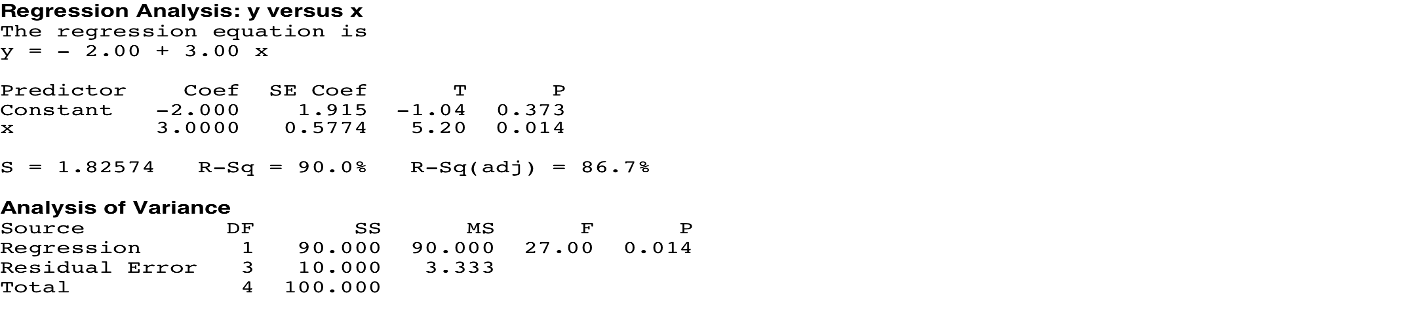
\includegraphics[width=1\textwidth]{img/5_RegOut.png}
%    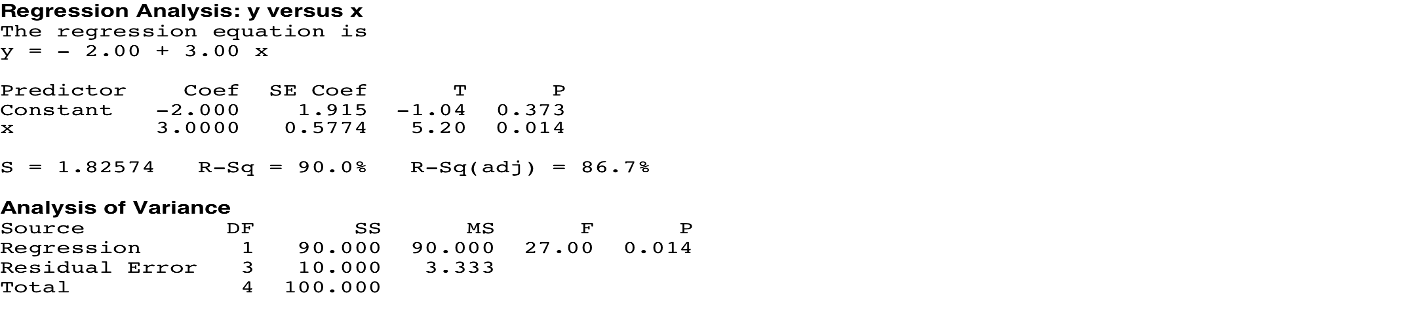
\includegraphics{img/5_RegOut.png}

    {\bf Regression Analysis: y versus x}\\
    \verb|The regression equation is|\\
    \verb|y = - 2.00 + 3.00 x|\\
    \verb||\\
    \verb|Predictor     Coef   SE Coef         T       P|\\
    \verb|Constant    -2.000     1.915     -1.04    0.373|\\
    \verb|x           3.0000    0.5774      5.20    0.014|\\
    \verb||\\
    \verb|s = 1.82574    R-sq = 90.0%    R-Sq(adj) = 86.7%|
    \verb||\\

    {\bf Analysis of Variance}\\
    \verb|Source           DF         SS        MS        F        P|\\
    \verb|Regression        1     90.000    90.000    27.00    0.014|\\
    \verb|Residual Error    3     10.000     3.333|\\
    \verb|Total             4    100.000|\\



    \begin{table}[ht]
      \Huge
      %\centering
      \begin{tabular*}{12cm}[h]{cc|c||cc||cc}
      Hours & Score & Predicted & Error & $($Error$)^2$ & Residual &  $($Residual$)^2$\\
      $x$ & $y$ & $\hat{y}$ & $y - \bar{y}$& $(y - \bar{y})^2$&  $y-\hat{y}$ &  $(y-\hat{y})^2$\\
      1 & 2 & \quad & &&&\\
      2 & 4 & \quad & &&&\\
      3 & 6 & \quad & &&&\\
      4 & 8 & \quad & &&&\\
      5 & 15 & \quad & &&&
      \end{tabular*}
      \end{table}

  % subsection subsection_name (end)
\newpage

  %%%%%%%%%%%
  %MAIN 4%%%%
  %5_3_Notes%
  %%%%%%%%%%%

  \section{The Correlation Coefficient $r$} % (fold)
  \label{}
  \subsection{Getting $r$}
  \begin{itemize}
    \item {\Huge $r = \frac{\Sigma z_x\cdot z_y}{n-1}$}
    \item Never calculate by hand; use calculator or computer output.
    \item Know formula {\em properties}.
  \end{itemize}
  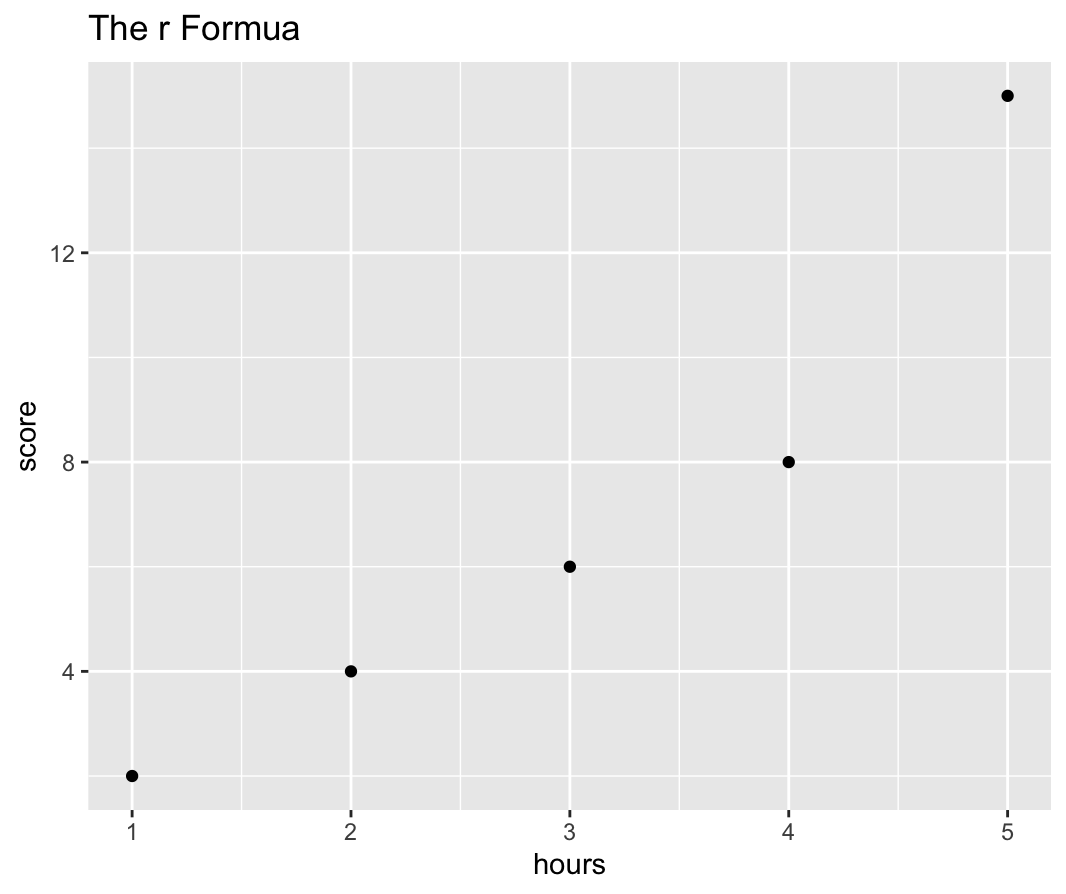
\includegraphics[width=.8\textwidth]{img/5_1_r_plot}\\[.3in]

  \begin{minipage}[T]{.45\textwidth}
    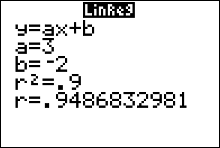
\includegraphics[width=.35\textwidth]{img/5_r}
  \end{minipage}
  \begin{minipage}[T]{.45\textwidth}
    {\bf Correlations: x, y }\\
    \verb|Pearson correlation of x and y = 0.949|\\
    \verb|P-Value = 0.014|
  \end{minipage}
  \vspace{1.5in}
  \subsection{Five R Properties} % (fold)
  \label{sub:5_r_properties}
  \begin{itemize}
    \item Examples
  \end{itemize}
  % subsection 5_r_properties (end)





\end{document}
